\section{UPPAAL modelling}\label{sec:sprint3-uppaal}
To illustrate how the UDP protocol should work in detail a UPPAAL model was constructed consisting of two templates: The host and an arbitrary amount of clients.
This first iteration of the model is not intended for heavy model checking, but rather to take a higher-level look at how the protocol is intended to work.
The two templates can be seen on Figures \ref{fig:uppaal-host-1} and \ref{fig:uppaal-client-1}.

\begin{figure}[H]
   \centering
    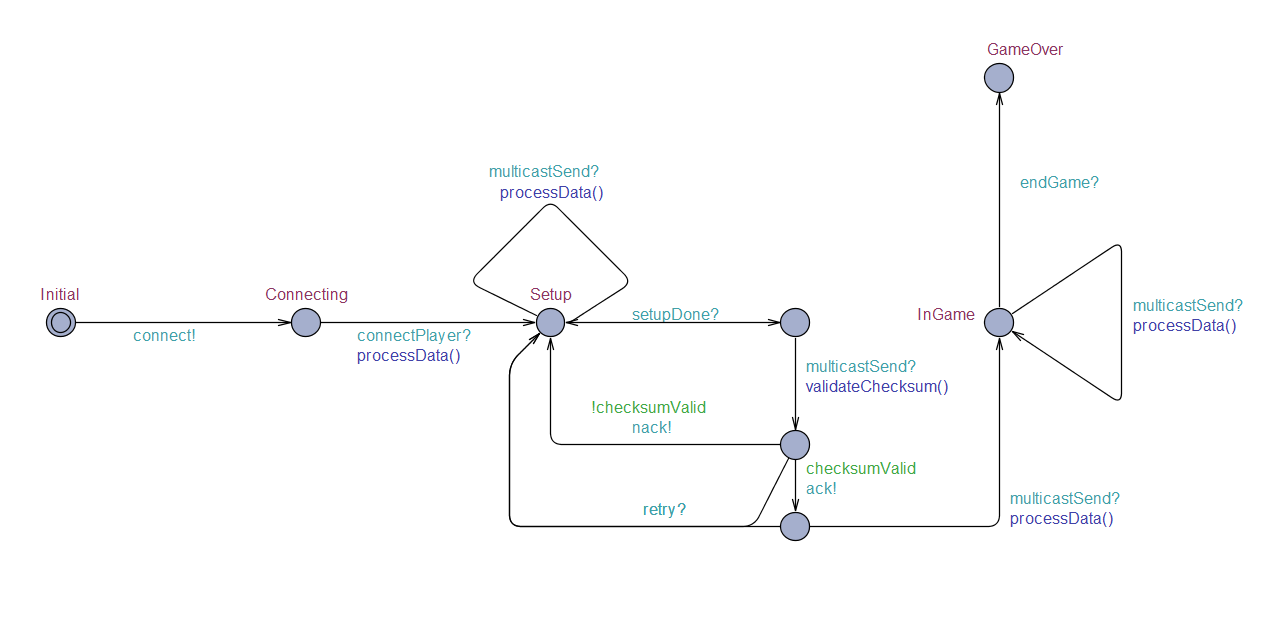
\includegraphics[width=1\linewidth]{/uppaal/client1.png}
    \caption{First iteration of the UPPAAL client template.}
    \label{fig:uppaal-client-1}
\end{figure}

\begin{figure}[H]
   \centering
    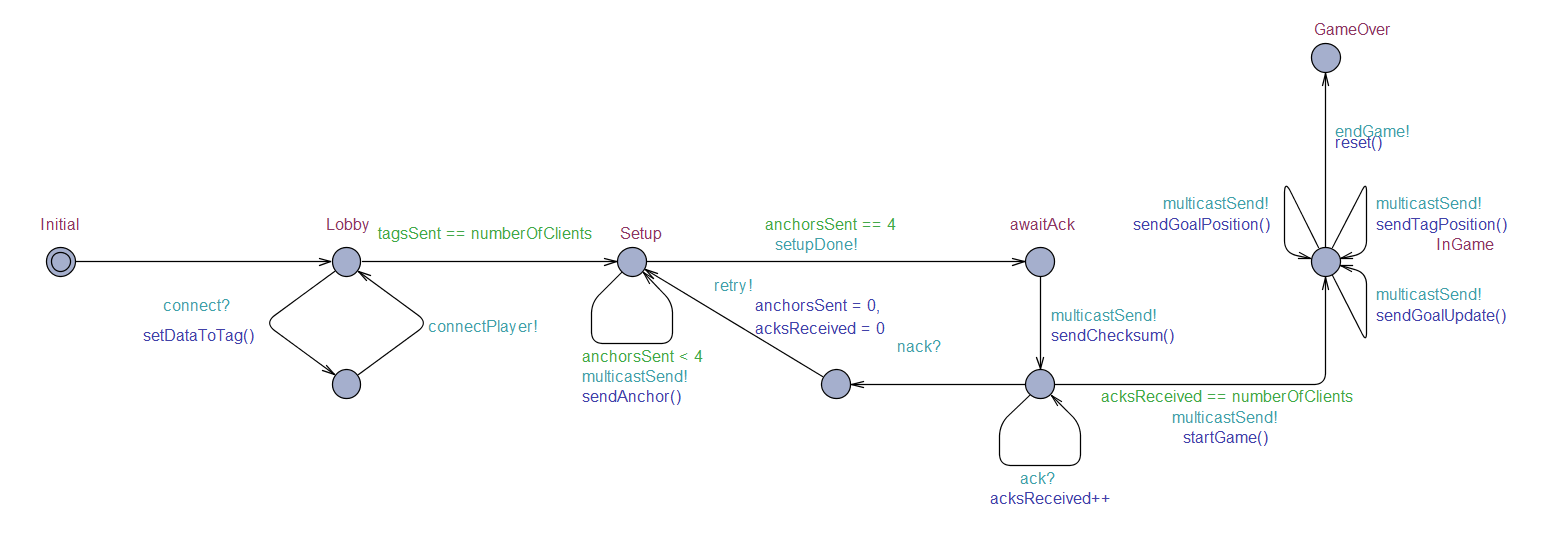
\includegraphics[width=1\linewidth]{/uppaal/host1.png}
    \caption{First iteration of the UPPAAL host template.}
    \label{fig:uppaal-host-1}
\end{figure}

\subsection{Walkthrough of the model}
The model for the client is fairly straight forward, it starts in an \uppLoc{initial} location which indicates that the client is not yet trying to connect to the host.
The connection happens on the edge from the initial location to the \uppLoc{connecting} location.
In the model, this is represented with the client utilizing the channel \uppChan{connect}, and waiting for the host to synchronize by listening to the same channel.
When the synchronization happens, the host will execute the \uppFunc{setDataToTag()} function, which updates the data it is transmitting, and uses the channel \uppChan{connectPlayer} to inform the client that connection is now ready.
The client will call a function \uppFunc{processData()} to read the content of the buffer and react accordingly. 
These steps will happen until the amount of \uppVar{tagsSent} is equal to the number of clients specified in the configuration.

\subsubsection{Setup}
The next location for both the host and client is \uppLoc{Setup}, which is the point where the host will transmit the anchor positions and ensure that all clients have consistent data.
The host will attempt to send the anchors one at a time with the \uppFunc{sendAnchor()} function until it has sent all 4 anchors to the clients.
Unlike the \uppChan{connect} and \uppChan{connectPlayer} channels, this happens on a broadcast channel, which allows multiple clients to receive the data at once to simulate the use of multicasting.
Since there is a chance that not all clients have received the four anchor coordinates correctly, the host will broadcast a checksum and have the clients either acknowledge or negative-acknowledge that the checksum is equal to the checksum of the data they have received.
In case any client returns a negative-acknowledge (using the channel \uppChan{nack}), all clients will go back to the setup and receive the anchor coordinates again until all clients send acknowledgements.

\subsubsection{InGame}
Finally, both the client and host will go to the \uppLoc{InGame} location to imply that the game is now happening.
To simulate asynchronous tasks, the host will continuously take a non-deterministic choice between sending a goal position, a tag position, a goal update or ending the game.
Meanwhile, the client only has two choices: Process data received on the multicast or wait for the game to end.

\subsubsection{Code aspect}
Behind the model, there are a series of variables and functions to make it all work.
In the global declarations the number of clients is specified, as well as an integer array called data, which is used as a buffer to transmit data between the host and clients, to simulate the internet connection in the real implementation.
The array has space for 5 elements to conform to the data format specified in \autoref{subsec:data-format}, such that the first element in the array will always be the type, which allows the client to act based on that when \uppFunc{processData()} is called.
The concrete implementation of \uppFunc{processData()} can be seen on \autoref{lst:uppaal:processData}.
For this iteration of the UPPAAL model, updating player and goal positions are not implemented, since it did not seem like a significant detail to model.

\begin{uppaalcode}[caption={Processing Data in UPPAAL model}, captionpos=b,label={lst:uppaal:processData}]
void processData(){
    int type = data[0];
    
    if(type == 0){
        int anchorId = data[1];
        anchorsX[anchorId] = data[2];
        anchorsY[anchorId] = data[3];
        anchorsReceived++;
    } else if(type == 1){
        // Player position
    } else if(type == 2){
        // Goal position
    } else if(type == 3){
        // Score update
    } else if(type == 4){
        // Tag received
        tag = data[1];
        playerId = data[2];
    } else if(type == 5){
        // Setup checksum
    } else if(type == 6){
        // Start game
    }
}
\end{uppaalcode}
\noindent
Likewise, when the host has to send data, it will update the first element of the buffer and fill in the relevant data in the other elements.

\subsubsection{Checksum}
A checksum will be calculated on the client for checking whether or not the client has the correct setup information, and based on the checksum that the host broadcasts, the players will return either an acknowledge or negative-acknowledge.
\\
This checksum is simply calculated as the sum of all four anchor coordinates, as seen in \autoref{lst:uppaal:checksum}.

\begin{uppaalcode}[caption={Calculating checksum in UPPAAL model}, captionpos=b,label={lst:uppaal:checksum}]
    void sendChecksum(){
        int checksum = 0;
        int i;
        for(i = 0; i < 4; i++){
            checksum += anchorsX[i];
            checksum += anchorsY[i];
        }
        data[0] = 5;
        data[1] = checksum;
    }
\end{uppaalcode}

\subsection{Updates to the network protocol}\label{subsec:sprint3networkupdate}
A good side-effect of generating the UPPAAL model was that it required some reflection upon the network data format specified in \autoref{subsec:data-format}.
This resulted in some minor refactoring of the format.
\\
First of all, the format for sending a field anchor position had a timestamp as a part of the package. 
Since the anchors will only be sent once, it does not make sense to timestamp it and this has been removed.
The updated version of the data format can be found in \autoref{app:network}
\\
Additionally, three new packages have been specified: Sending a player tag, sending an acknowledgement or sending the signal to start the game.

\begin{table}[h!]
    \centering
    \begin{tabular}{|l|l|l|}
    \hline
    \begin{tabular}[c]{@{}l@{}}PLAYER\_ID (p)\\ (1-4)\end{tabular} & \begin{tabular}[c]{@{}l@{}}TAG\_ID (i)\\ (0-65.535)\end{tabular} & TYPE (t) \\ \hline
    8 bits                                                         & 16 bits                                                          & 8 bits   \\ \hline
    \end{tabular}
    \caption{Format sending player tag.}
    \label{tab:player-tag}
\end{table}

\begin{table}[h!]
    \centering
    \begin{tabular}{|l|}
    \hline
    \begin{tabular}[c]{@{}l@{}}ACK (a)\\ (0-1)\end{tabular} \\ \hline
    8 bits                                                  \\ \hline
    \end{tabular}
    \caption{Acknowledge or negative-acknowledge.}
    \label{tab:acknowledge}
\end{table}

\begin{table}[h!]
    \centering
    \begin{tabular}{|l|}
    \hline
    \begin{tabular}[c]{@{}l@{}}TYPE (t)\\ 6\end{tabular} \\ \hline
    8 bits                                               \\ \hline
    \end{tabular}
    \caption{Game start.}
    \label{tab:gamestart}
\end{table}
\noindent
The reason that \autoref{tab:acknowledge} does not have a type is that it is the only package that will be sent from the client to the host, so it will only need to contain a signal for the host to know whether the checksum is correct or not.
